
%%%%%%%%%%%%%%%%%%%%%%%%%%%%%%%%%%%%%%%%%%%%%%%%%%%%%%%%%
% The original template for this document was taken from:
% http://www.michaelshell.org/tex/ieeetran/
%
% Adapted for courses at the University of Regina by:
% Mikhail Shchukin 
%
% Edited by Trevor Tomesh
% October 20th 2019
%%%%%%%%%%%%%%%%%%%%%%%%%%%%%%%%%%%%%%%%%%%%%%%%%%%%%%%%%

%!!!!!!!!!!!!!!!!!!!!!!!!!!!!!!!!!!!!!!!!!!!!!!!!!!!!!!!!
%!!!!!!!!!!!!! DON'T TOUCH THIS !!!!!!!!!!!!!!!!!!!!!!!!!
\documentclass[journal,onecolumn]{IEEEtran}
\usepackage{graphicx}
\usepackage{placeins}
\usepackage{mathtools}
\usepackage{listings}
\usepackage{threeparttable}
\usepackage{subfigure}
\graphicspath{ {./img/} }
\hyphenation{op-tical net-works semi-conduc-tor}
\begin{document}
%!!!!!!!!!!!!!!!!!!!!!!!!!!!!!!!!!!!!!!!!!!!!!!!!!!!!!!!!!
%!!!!!!!!!!!!!!!!!!!!!!!!!!!!!!!!!!!!!!!!!!!!!!!!!!!!!!!!!


% Enter the course, assignment number, your name, and student ID below: 
\newcommand{\course}{CS 490DB} % course
\newcommand{\anum}{} % assignment number
\newcommand{\name}{Carl F. Sandin} % your name
\newcommand{\sid}{200375294} % student ID


%!!!!!! DON'T TOUCH THIS !!!!!!!!!!!!!!!!!!!!!!!!!!!!!!!!!!
\title{\course{} \\ Research Paper \ \anum{}}
\author{\name{},~\IEEEmembership{\course{},~University~of~Regina},~Student ID\# \sid{}}
\maketitle
%!!!!!!!!!!!!!!!!!!!!!!!!!!!!!!!!!!!!!!!!!!!!!!!!!!!!!!!!!!


\section{Abstract}
With climate change discussions becoming more prevalent, this paper aims to observe a correlation between land types and carbon emissions. The assumption is that with increasing land types, such as forestry, the amount of needed land to equalize carbon emissions will go down, a negative correlation. This study takes five countries and notes their total land make-up, including, but not limited to, crop land, forestry, fishing, and urban infrastructure. With these variables taken into account, the trend moves towards a positive correlation, opposite of our previous assumptions.


\section{Known Issues and Limitations}
This program has a run time complexity of $O(n^2)$. This can be very tasking when dealing with larger data sets. If this study was conducted longer, or had more incremental measures, the program would struggle to compute.
\\  Further, since the data sets only survey five economically viable countries, data could have different results. If all countries in the ledger provided could be analyzed into a meta-data study, it may produce a different result.

\section{Problem Statement}
The issue around carbon emissions and climate change can be complex. There is an overwhelming amount of variables that could be affecting the carbon footprint. One variable that may assist in reducing the carbon emissions is more plotted land. If there is more land, there could be more forestry, plants, and other factors to reduce carbon emissions. The goal of the graphical models is to see if, when total land per country increases, then carbon emissions will reduce as well.
 
\section{Background}
\subsection{Data File}
The data file used for this analyze was posted by the Global Footprint Network as a comma separated value file on the website Kaggle \cite{national:2018}. The data has many interesting data points, that includes the United Nations regions and sub-regions, population, GDP, land types, and other factors. The data spans from 1960 to 2014, with some variable years depending on country, and has 196 countries in the list, equalling 87020 rows of data.
\subsection{Data Hypothesis} 
Many people would assume the more forests we have, the more carbon will be reduced in the atmosphere. When I found this data set, I found this to be a presentable opportunity to test that hypothesis. As noted in the abstract, this may not be the case, or there are stronger factors than the land versus the carbon emissions. If the land masses cannot keep up to the demand for carbon consumption, then countries may need to re-evaluate priorities or concerns.
\subsection{Additional Notes}
Along side the main argument, a second graph detailing population over time will be presented underneath the main graph. This is so the reader can have a reference to deduce whether population increase may correlate with the data. 

\newpage

\section{Model Development}
    When developing my models, I found it insufficient to observe one country. I took five at pseudo-random, choosing a country from each continent. On a smaller level, I wanted myself and any future readers to note if the continent had any factor in the results. Of these five countries, I took their 539 data entries of total land, land needed for carbon equilibrium, population and recorded year. Further, I trimmed the zero or null elements of the carbon list, as they were missing or unrecorded data entries, from all the lists. This left me with four list of lists to implement in our machine learning algorithm.
    
\newline As most of the graphs observed followed a linear trend, I found it appropriate to implement the {\it LinearRegression()} algorithm. This is done by first by declaring regression models by making them equal to {\it LinearRegression()}. For the algorithm to accurately read data, we have to reshape the list of lists to be readable by the function. we can use the {\it .reshape()} appendix to our array using the panel data plug-in. {\it .fit()} is how we train the model; with what x is plugged in, and what y outcome is made, it 'learns' and tries to predict the y outcomes based on x. We use these predictions to create our line of best fit, which is then plotted as the linear regression line.

     \begin{figure}[h]
	\centering
  	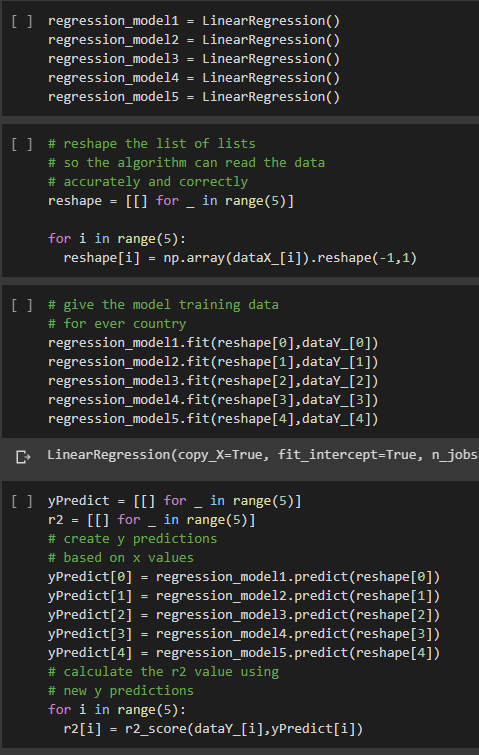
\includegraphics[width=0.5\textwidth]{img/Model-Dev.png}
    \centering
    \caption{ Process for implementing the machine learning algorithm}	
  	\label{fig:MLA}
\end{figure}\\

\\* Finally, using all this data, we can calculate the $R^2$ score. This helps us see the error margin between what the line would have predicted as the y-value, and the actual y-value. The closer $R^2$ gets to 1, the closer the actual y-value is to the y-prediction. This means the points correlate correctly.

\newpage

\section{Model Evaluation}

From the models depicted of our results, it seems most have a strong correlation upwards. This disproves our initial thesis on the correlation of data points. Most graphs have an $R^2$ value above .9, indicating a strong growth. This concludes that there may be stronger factors at play; with the growth of land, hectares needed still increases. The two unique differences between the other sets, however, show:
\begin{itemize}
\item While every other country had a steady population growth, Japan's growth started to level between 1990 and 2000.
\item Nigeria significantly drops and is able to keep the hectares needed fairly low, until later in the half-decade.
\end{itemize}

This can indicate the start of the shortcomings of these models, The first being a small sample size. If we were to observe and record the findings of every country, we could group similar growth rates together and see what factors those countries had during those periods. The second limitation to this model is missing the variables given. Since total land also includes human infrastructure, the metropolitan areas can contribute to a larger demand of carbon in that country. The downside is that forests rarely get larger, only smaller compared to cities. A better way to accurately portray results is to split each type of land into it's own category and observe their differences. due to the size and vastness of this objective, it is not possible for me, but I hope to have someone try to explore this possibility.

\newline
On the optimistic side, we can see some sort of trend between the two variables. There is a relationship there to be found, and means there is more studying to be done. With the nature of science, there is always ways to interpret data, and there is more to interpret than what is shown on the surface level of this model.

\section{Concluding Remarks}

We aimed to find a negative correlation between the amount of total land per country and the amount of land needed to achieve zero net carbon emissions. With the graphical data presented in Appendix A and the machine learning algorithm, we are shown this is not the case. However, there is some sort of relationship between the data points, and with further analysis we may be able to find a root cause. For this model, this is important because the world is our home. We develop land and take land away for resources, but we must know the implications of what is being caused by these actions. On the broader sense, having machine learning depict relationships between data points helps us ask the proper questions for issues such as this. Having these tools so readily available means questions such as the one I presented may one day have a conclusive answer.

\newpage

\appendices

\section{Graphical Models}

\subsection{\centering Canada}
     
     \begin{figure}[h]
	\centering
  	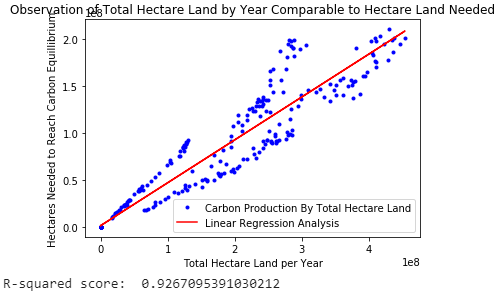
\includegraphics[width=0.7\textwidth]{img/Canada-Carbon.png}
  	  	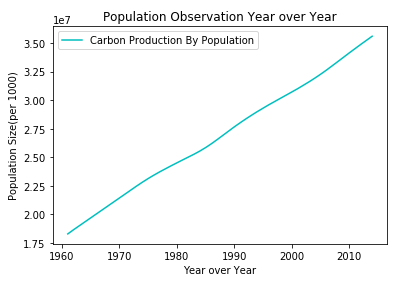
\includegraphics[width=0.7\textwidth]{img/Canada-Population.png}
\end{figure}\\



\newpage

\subsection{\centering Japan}
     
     \begin{figure}[h]
	\centering
  	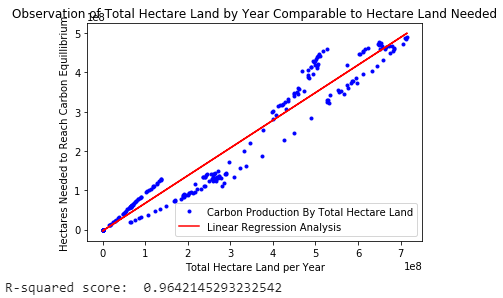
\includegraphics[width=0.7\textwidth]{img/Japan-Carbon.png}
  	  	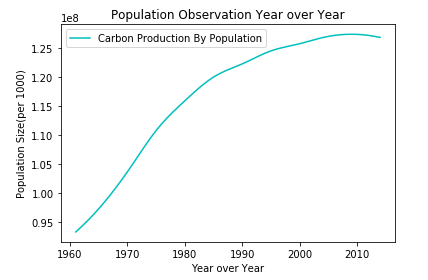
\includegraphics[width=0.7\textwidth]{img/Japan-Population.png}
\end{figure}\\

\newpage

\subsection{\centering Ireland}
     
     \begin{figure}[h]
	\centering
  	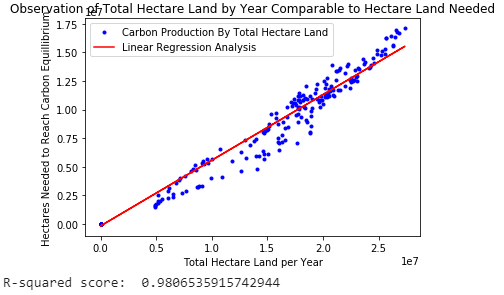
\includegraphics[width=0.7\textwidth]{img/Ireland-Carbon.png}
  	  	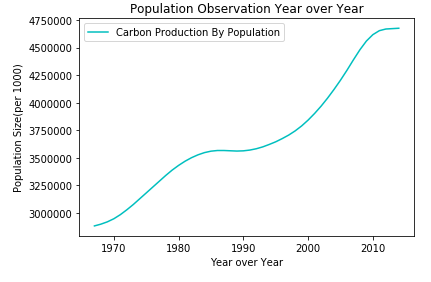
\includegraphics[width=0.7\textwidth]{img/Ireland-Population.png}
\end{figure}\\

\newpage

\subsection{\centering Nigeria}
     
     \begin{figure}[h]
	\centering
  	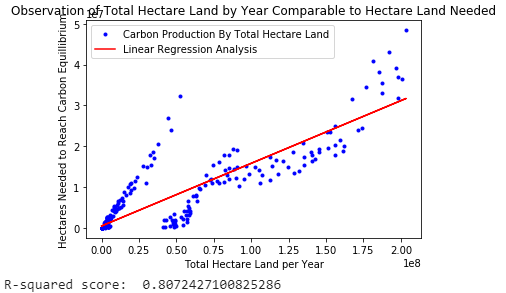
\includegraphics[width=0.7\textwidth]{img/Nigeria-Carbon.png}
  	  	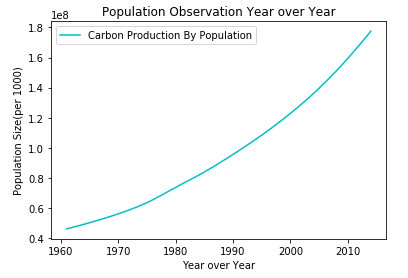
\includegraphics[width=0.7\textwidth]{img/Nigeria-Population.png}
\end{figure}\\

\newpage

\subsection{\centering Australia}
     
     \begin{figure}[h]
	\centering
  	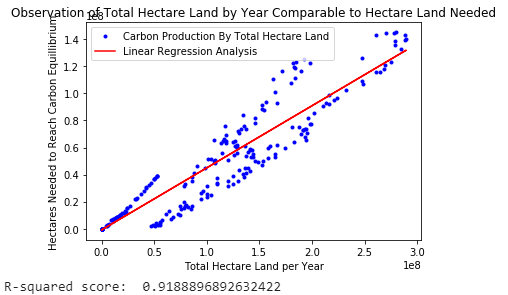
\includegraphics[width=0.7\textwidth]{img/Australia-Carbon.png}
  	  	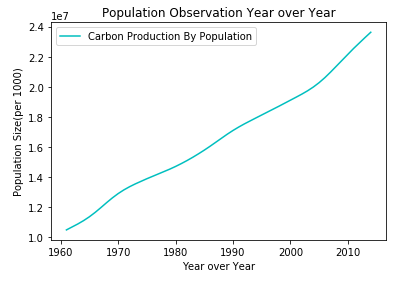
\includegraphics[width=0.7\textwidth]{img/Australia-Population.png}
\end{figure}\\

\newpage

\section{cfs\_research\_notebook.py}
\label{app1}
\lstset{basicstyle=\small\selectfont\ttfamily}
\lstinputlisting[language= python, 
breaklines=true,         
showtabs=false,
showstringspaces=false,
numberstyle=\tiny\color{mygray}
caption={The raw code for this assignment},
captionpos=b,label=lst2]{cfs_research_notebook.py}

\newpage


\begin{thebibliography}{1}


\bibitem{national:2018}
National Footprint Accounts 2018. (2019). Retrieved 6 December 2019, from https://www.kaggle.com/footprintnetwork/national-footprint-accounts-2018

\end{thebibliography}

% this is the end of all
\end{document}
